\subsection{Image and text: a controlled proof of concept}
\label{sec:exp:imagetext}

We use image--text as a controlled proof of concept for the interface rather than as a
natural-image benchmark. MNIST-Sum pairs four binarised MNIST digits \citep{image:mnist} with
their ordered equation and sum, so every direction has an exact answer: read and add a supplied
image, draw four named digits from a supplied equation, or generate an image and an equation that
agree. The task is not included because MNIST is difficult. It is included because every
conditional and joint direction is exactly auditable, which lets us show that raw visual bits and
symbolic text bits form a learnable joint generative space under one modality-agnostic 1-D
denoiser.

\begin{figure}[t]
\centering
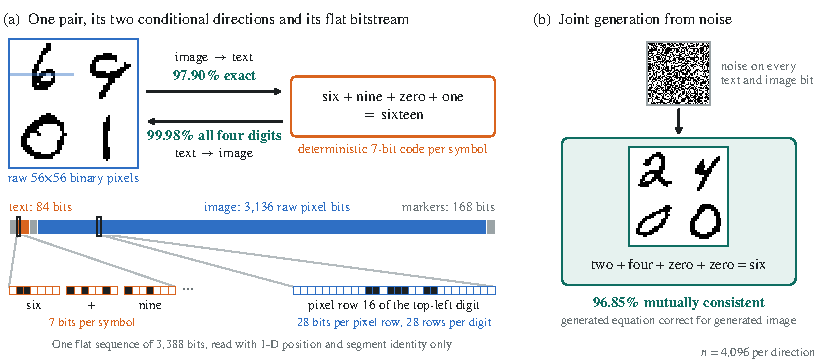
\includegraphics[width=\linewidth]{figures/mnist_sum/fig_mnist_sum_compact.pdf}
\caption{MNIST-Sum, an exactly auditable image--text control. (a) Four binarised MNIST digits and
their equation are written as one flat sequence of 3,388 bits: 3,136 raw pixel bits, 84 text
bits (twelve deterministic 7-bit symbol codes) and 168 marker bits, so neither side has a learned
tokenizer; the zoom-ins show actual bits of this pair. One 63.3M-parameter denoiser serves both conditional
directions by observing one half of the stream and denoising the other. Image$\rightarrow$text is
scored by exact string match; text$\rightarrow$image requires a fixed quadrant classifier to
recover all four requested digit identities. (b) With nothing observed, the same weights
co-generate an image and an equation from noise; a sample counts only if the generated equation
is correct for the generated image. Rates are over $n{=}4{,}096$ samples per direction; the
samples shown are fixed examples that illustrate, rather than estimate, these rates.}
\label{fig:mnist:sum}
\end{figure}

\textbf{One bitstream, no learned tokenizer.} Images enter as raw binary pixels and text as a
deterministic 40-symbol, 7-bit code; a pair becomes one flat sequence of 3,388 bits (3,136 pixel
bits, 84 text bits and 168 marker bits), which the denoiser reads in 28-bit positions. It receives
this flat sequence, its 1-D position and segment identity, but no pixel grid, 2-D attention structure, image encoder, text encoder or
modality-specific head. A single 63.3M-parameter model trained for 500K steps performs all three
directions; only the observed part of the stream changes.

\textbf{Result.} At $n{=}4{,}096$ per direction, image$\rightarrow$text is 97.90\% exact,
text$\rightarrow$image places all four requested digits correctly in 99.98\% of samples, and
joint co-generation from noise is 96.85\% mutually consistent (Figure~\ref{fig:mnist:sum}).
Held-out digit tuples reach 97.92\% image$\rightarrow$text, statistically indistinguishable from
seen tuples. The qualitative samples in the figure only illustrate these rates; the evidence is
the aggregate evaluation. Appendix~\ref{app:image:mnist} gives classifier calibration, confidence
intervals and the error decomposition. Having established the interface where it can be audited
exactly, the remaining experiments turn to the serious higher-scale settings: audio--text
(\S\ref{sec:exp:audio}) and protein sequence--structure (\S\ref{sec:exp:protein}).

\FloatBarrier
